\documentclass[twoside]{article}
\usepackage{preamble}
\usepackage{subcaption}
\begin{document}

\maketitle % Insert title

\thispagestyle{fancy} % All pages have headers and footers

%----------------------------------------------------------------------------------------
%	ABSTRACT
%----------------------------------------------------------------------------------------

\begin{abstract}
PIC-simulation of supersonic plasma flow around two different objects, a rectangle and a cylinder, have been conducted, with various plasma and magnetic field parameters. For the rectangle, cone angles were observed to be in good agreement with theory. For the cylinder, simulated with a magnetic field of different angles of attack, asymmetry in the wake was observed, as anticipated.
\end{abstract}

%-----------------------------------------------------------------------------------
%	ARTICLE CONTENTS
%-----------------------------------------------------------------------------------

\begin{multicols}{2} % Two-column layout throughout the main article text

\section{Introduction}

\lettrine[nindent=0em,lines=2]{I}n the following article we will explore plasma-spacecraft interaction by using particle-in-cell (PIC) model.
The study is conducted to further expand our knowledge on the interplay of sounding rockets and the surrounding ionospheric plasma and its effect on the spacecraft by using numerical methods. Of the effects we are looking for, a.l., is the effect of the plasma flow on the rocket, and the instruments in particular. More distinctly, our field of interest is the wakefield arising behind the object and furthermore the electron and ion density within the wake region and the electrical potential surrounding the body. \\
\indent There have been many studies in the fields of computational plasma physics ranging from dusty plasmas and objects immersed in flowing plasmas. Melandso and Goree \cite{melandso} study the polarisation effects behind a particle immersed in a plasma at supersonic speed. The same simulation was run with two aligned particles studying the collective effect, which could be relevant for our studies, considering the effect of possible plasma wakes between probes. Simulation performed by Wang and Hastings \cite{wang} show how the plasma wake arising behind the object is affected by the electrical charge of the body, this can be shown to affect the electronics on-board the spacecraft. \\
\indent We base our model on the ICI-rockets, albeit much simplified. The ICI-rockets are to measure the electron density, electric field, potential and other physical quantities in the ionosphere. Consequently the results could be used to develop more suited materials.
%------------------------------------------------
% COMMENTS ON THE  ABOVE
% Too much detail
% Almost like abstract
% numerical section
% the introduction is mixed with the other sections. 
% haven't mentioned the problem and vague no focus
% Motivation should come earlier not last 
% Beginning is ok
% can discuss further the charged spacecraft and how it modifies the flow
% Good thing to describe previous studies


\section{Numerical experiment}
 \lettrine[nindent=0em,lines=2]{O}ur simulation will consist of a plasma flowing around an object of two different shapes. We will be using the three dimensional code developed by Kobe University and running it on the $\pi$-computer in Kobe, Japan. The code \cite{EMSES} (EMSES: Electro-Magnetic Spacecraft Environment Simulator = Full PIC code
  + Spacecraft/rocket body treatment) can perform both electrostatic and electromagnetic thus enabling us to see the different scenarios with and without the magnetic field including the alignment of the magnetic field in respect to the object. The PIC-model solves Maxwell's equation for fields and the equation of motion for particles in self-consistent manner. PIC is discretised using finite difference methods. \\
\indent The simulation consist of two parts, one with the rectangular and one with the cylinder, the first one taking place in Kobe and the second in Oslo, Norway. With the rectangular object, the code was run with a magnetic field of $B=0$ (i.e. no magnetic field) and $B=50\mu T$ parallell with the $z$-axis. % Without magnetic field with plasma flow velocity $M = 2$ at the inlet.
In both cases we used a plasma flow perpendicular to the rocket. Due to a misprint, the electrostatic case was simulated with a plasma speed of $M=20$ instead of $M=2$, which was the velocity we were aiming for. \\
\indent In Oslo, the simulation with the cylinder was conducted, this time three simultaneous simulations were run all with magnetic fields of the same strength as the previous case, with different angles with respect to the object, $0$, $45$ and $90$ degrees. Plasma flow speed in this case was also $M=2$.\\

\end{multicols}
\vspace{-3cm}
\section{Results}

% ion elec density rectangle, no B, M20
\begin{figure}[H]
\centering
\begin{subfigure}{.5\textwidth}
  \centering
  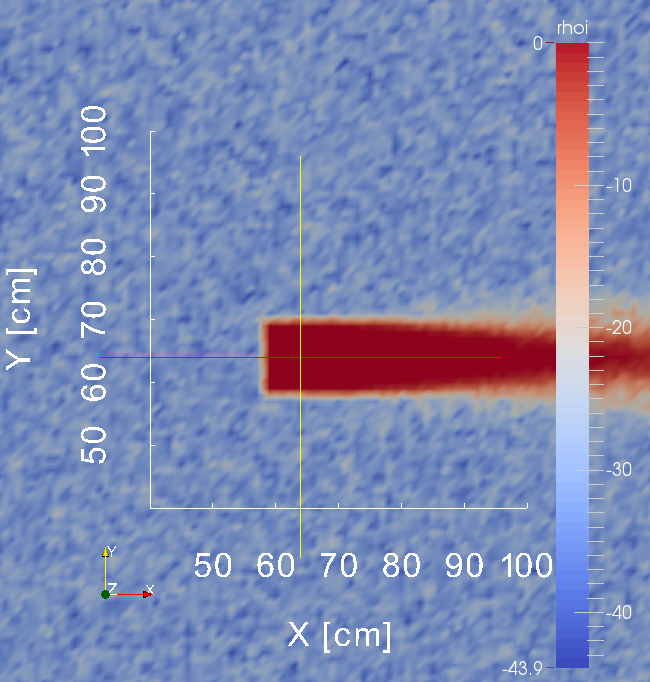
\includegraphics[width=\linewidth]{rhoi_xy_plane_nomag_M20.png}
  \caption{Ion density}
  \label{fig:sub11}
\end{subfigure}%
\begin{subfigure}{.5\textwidth}
  \centering
  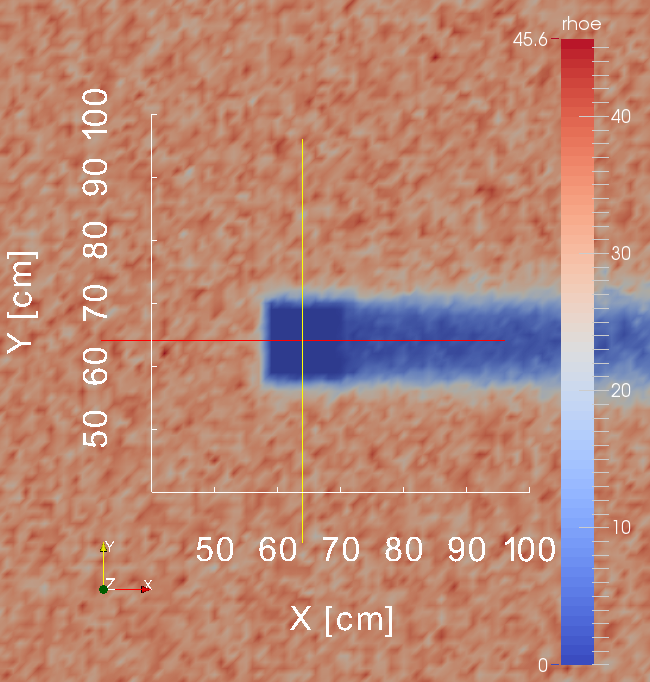
\includegraphics[width=\linewidth]{rhoe_xy_plane_nomag_M20.png}
  \caption{Electron density}
  \label{fig:sub12}
\end{subfigure}
\caption{Plots of ion density (a) and electron density (b) in the electrostatic case with Mach 20. A cut has been made through the center in the $xy$-plane. Due to the extreme velocity, the cone angle is very small, about 2.8 degrees.}
\label{fig:1}
\end{figure}

% ion elec density rectangle with B and M2
\begin{figure}[H]
\centering
\begin{subfigure}{.5\textwidth}
  \centering
  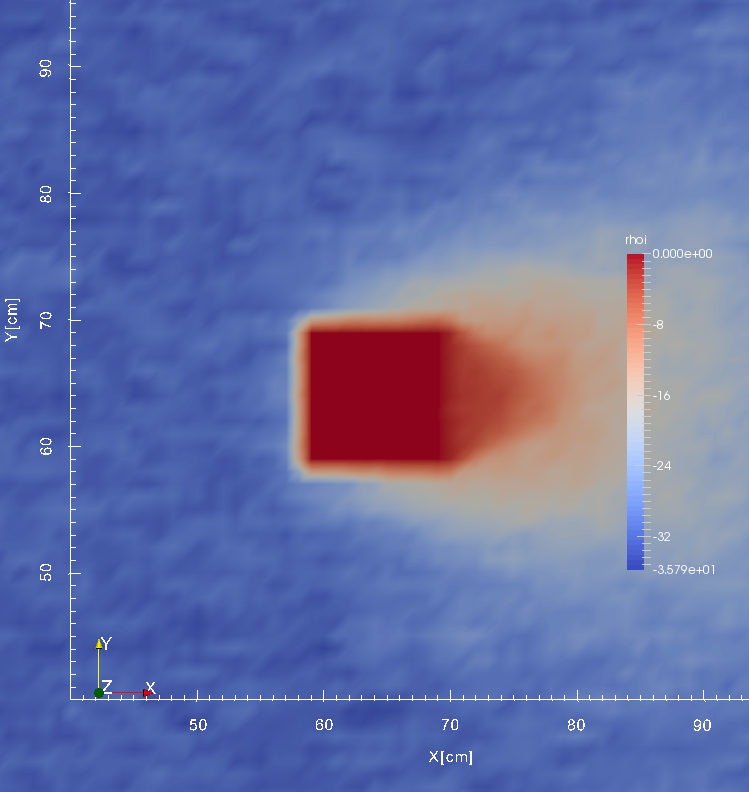
\includegraphics[width=\linewidth]{rhoi_1sim_kobe_M2_B50.png}
  \caption{Ion density}
  \label{fig:sub21}
\end{subfigure}%
\begin{subfigure}{.5\textwidth}
  \centering
  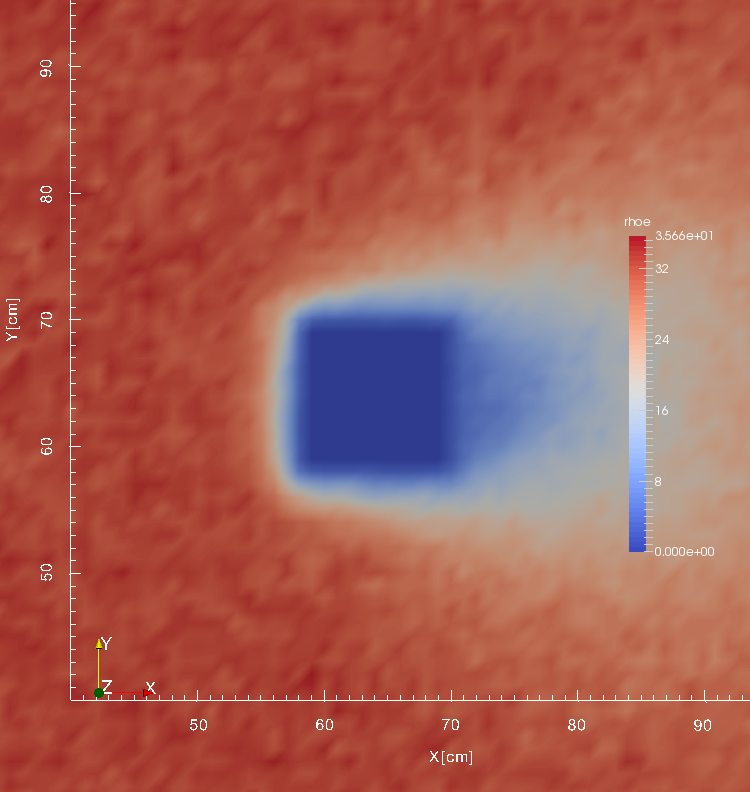
\includegraphics[width=\linewidth]{rhoe_1sim_kobe_M2_B50.png}
  \caption{Electron density}
  \label{fig:sub22}
\end{subfigure}
\caption{Simulation of rectangle with magnetic field parallel with the object's longitudinal direction and Mach number 2. A cut has been made through the center in the $xy$-plane. Theoretically the cone angle should be 30 degrees.}
\label{fig:2}
\end{figure}

% Potential rectangle M2 with B
\begin{figure}[H]
\centering
\begin{subfigure}{.5\textwidth}
  \centering
  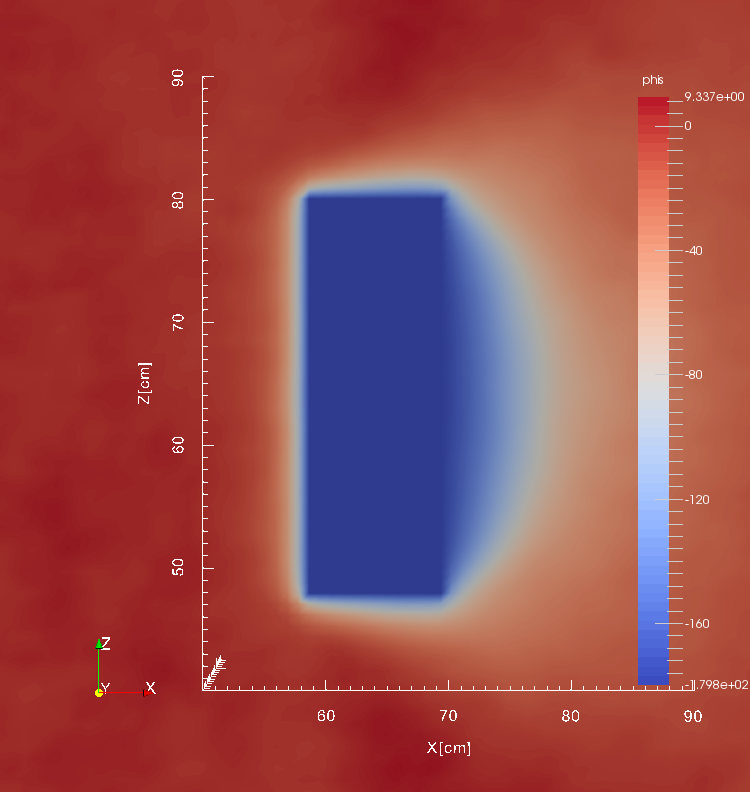
\includegraphics[width=\linewidth]{phis_1sim_kobe_B50.png}
  \caption{Electric potential}
  \label{fig:sub31}
\end{subfigure}%
\begin{subfigure}{.5\textwidth}
  \centering
  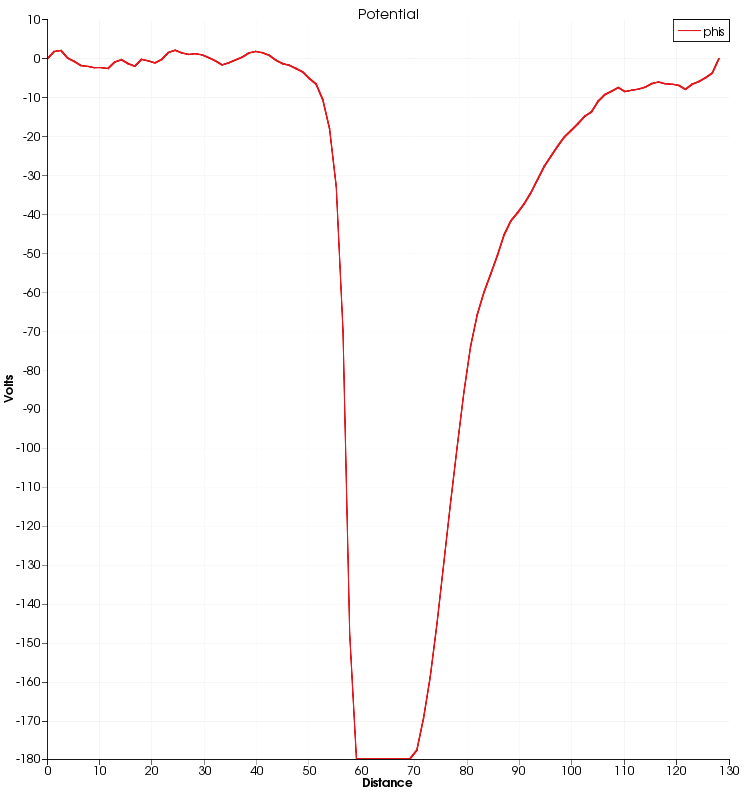
\includegraphics[width=\linewidth]{phispot_1sim_kobe_B50.png}
  \caption{Potential curve}
  \label{fig:sub32}
\end{subfigure}
\caption{Electric potential for a rectangel in a plasma flowing at $M=2$ and with magnetic field. (\ref{fig:sub31}) is made by doing a cut through the center in the $xz$-plane. (\ref{fig:sub32}) is made by taking a cut through the center of the rectangle parallell with the x-axis.}
\label{fig:3}
\end{figure}

% ion elec density, cylinder, B 0 deg, M2
\begin{figure}[H]
\centering
\begin{subfigure}{.5\textwidth}
  \centering
  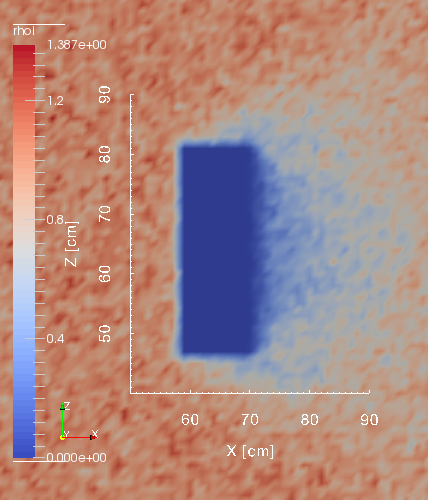
\includegraphics[width=\linewidth]{zoom/rhoi_Y(zoom).png}
  \caption{Ion density}
  \label{fig:sub41}
\end{subfigure}%
\begin{subfigure}{.5\textwidth}
  \centering
  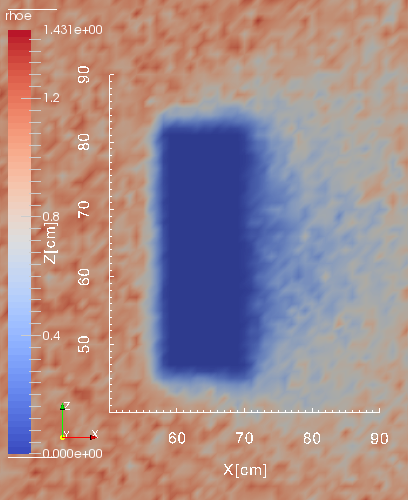
\includegraphics[width=0.955\linewidth]{zoom/rhoe_Y(zoom).png}
  \caption{Electron density}
  \label{fig:sub42}
\end{subfigure}
\caption{Simulation of cylinder with magnetic field parallel to cylinders longitudinal direction. Figure (\ref{fig:sub41}) and (\ref{fig:sub42}) shows the density of ions and electrons respectively. }
\label{fig:4}
\end{figure}

% Potential cylinder M2 B 0deg
\begin{figure}[H]
\centering
\begin{subfigure}{.5\textwidth}
  %\centering
  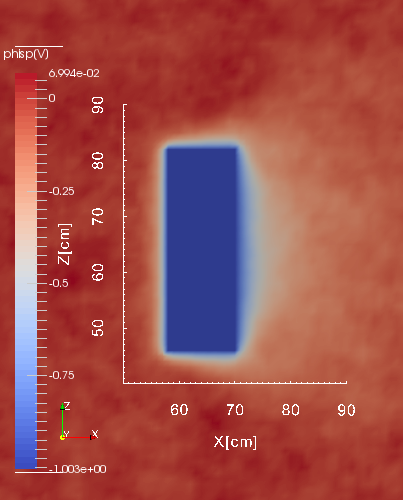
\includegraphics[width=0.8\linewidth]{zoom/phisp_Y(zoom).png}
  \caption{Electric potential}
  \label{fig:sub51}
\end{subfigure}%
\begin{subfigure}{.5\textwidth}
  %\centering
  \hspace{-13mm}
  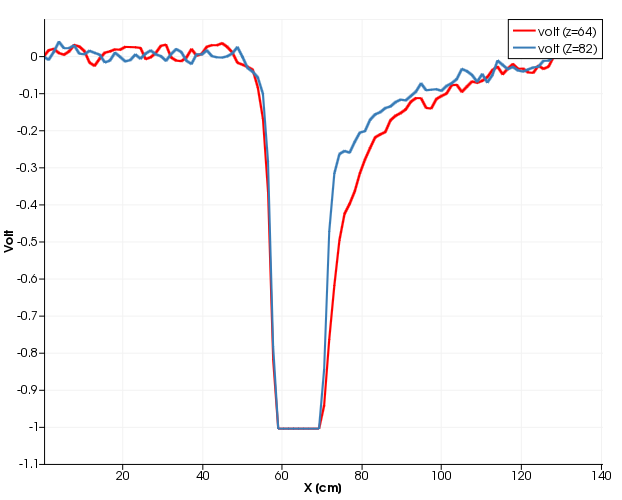
\includegraphics[width=1.2\linewidth]{zoom/plot_phisp(Z64Z82onphisp_Y).png}
  \caption{Potential along cut}
  \label{fig:sub52}
\end{subfigure}
\caption{Potential plots for cylinder with magnetic field parallel to the cylinder and $M=2$. The potential curves was made by taking cuts through the top and center of the cylinder, with blue and red color respectively.}
\label{fig:5}
\end{figure}

% ion elec density, cylinder, B 0 deg, M2
\begin{figure}[H]
\centering
\begin{subfigure}{.5\textwidth}
  \centering
  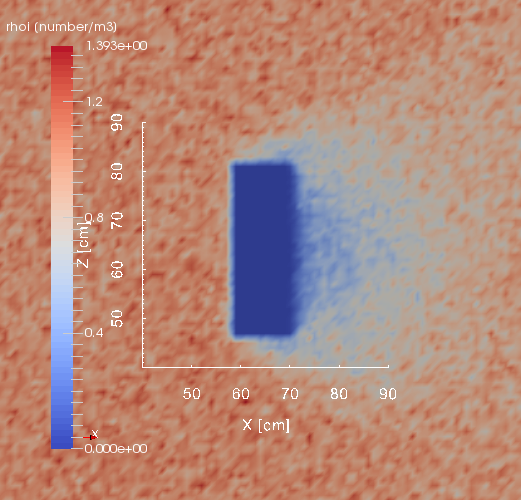
\includegraphics[width=\linewidth]{zoom_png/rhoi_zoom.png}
  \caption{Ion density}
  \label{fig:sub61}
\end{subfigure}%
\begin{subfigure}{.5\textwidth}
  \centering
  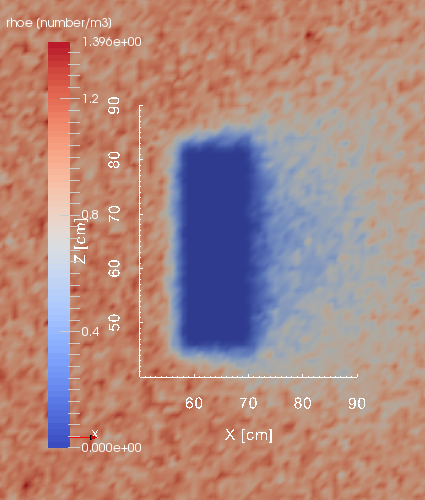
\includegraphics[width=0.8155\linewidth]{zoom_png/rhoe_zoom.png}
  \caption{Electron density}
  \label{fig:sub62}
\end{subfigure}
\caption{Simulation of cylinder with magnetic field at 45 degrees w.r.t the cylinder. Figure (\ref{fig:sub61}) and (\ref{fig:sub62}) shows the density of ions and electrons respectively. We can observe some asymmetry in the wake, due to the skewed magnetic field.}
\label{fig:6}
\end{figure}

% Potential cylinder M2 with B45
\begin{figure}[H]
\centering
\begin{subfigure}{.5\textwidth}
%  \centering
  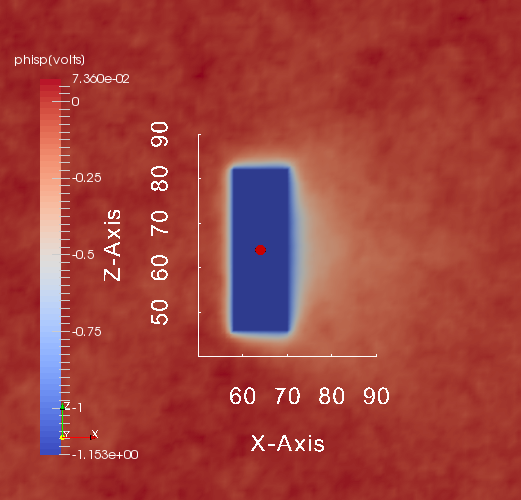
\includegraphics[width=0.85\linewidth]{zoom_png/phisp_zoom.png}
  \caption{Electric potential}
  \label{fig:sub71}
\end{subfigure}%
\begin{subfigure}{.5\textwidth}
%  \centering
  \hspace{-10mm}
  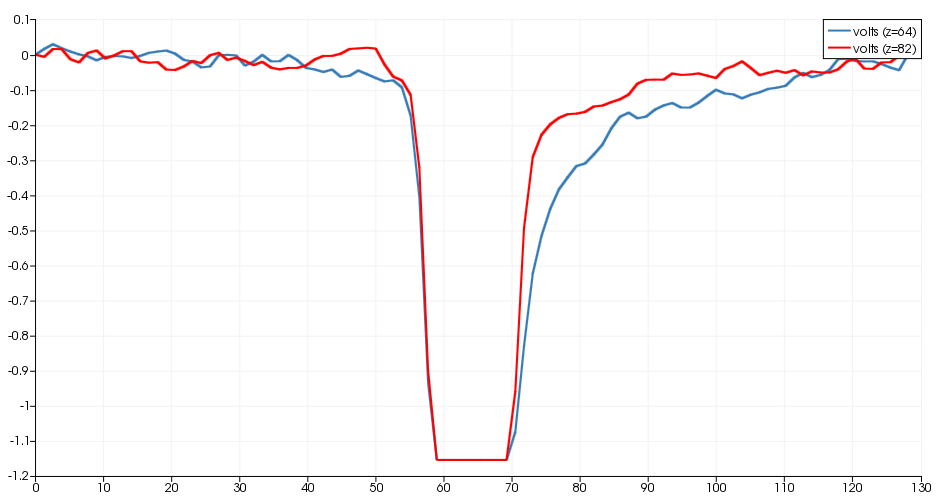
\includegraphics[width=1.2\linewidth]{cmp_phisp.png}
  \caption{Potential curve}
  \label{fig:sub72}
\end{subfigure}
\caption{Electric potential for a cylinder in a plasma flowing in the x-direction at $M=2$ and with a magnetic field at 45 degrees. (\ref{fig:sub72}) is made by taking a cut through the top and center (red and blue respectively) of the cylinder parallell with the x-axis.}
\label{fig:7}
\end{figure}

% ion elec density, cylinder, B90
\begin{figure}[h]
\centering
\begin{subfigure}{.5\textwidth}
  \centering
  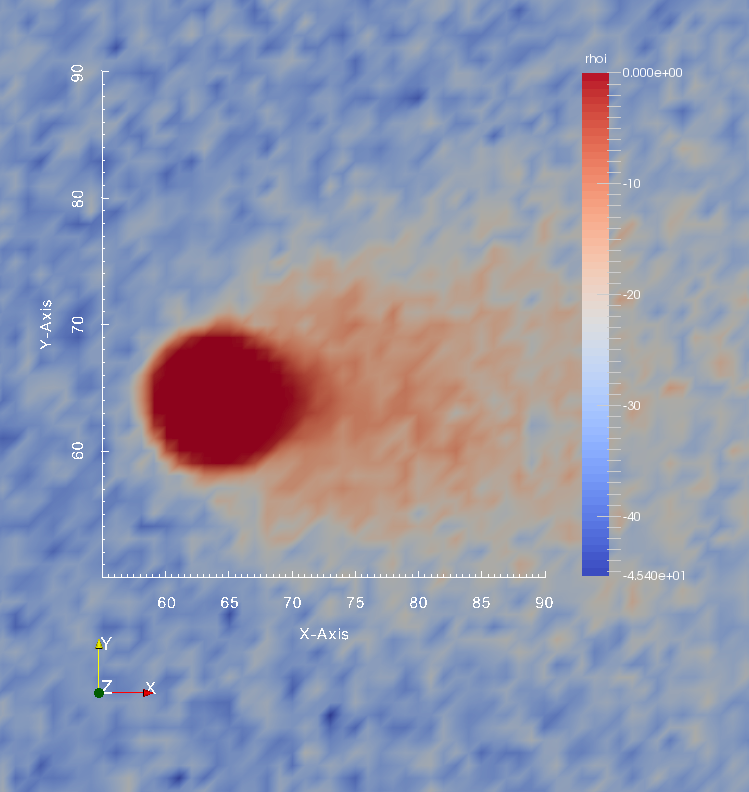
\includegraphics[width=0.99\linewidth]{rhoi_2sim_oslo_90D.png}
  \caption{Ion density}
  \label{fig:sub81}
\end{subfigure}%
\begin{subfigure}{.5\textwidth}
  \centering
  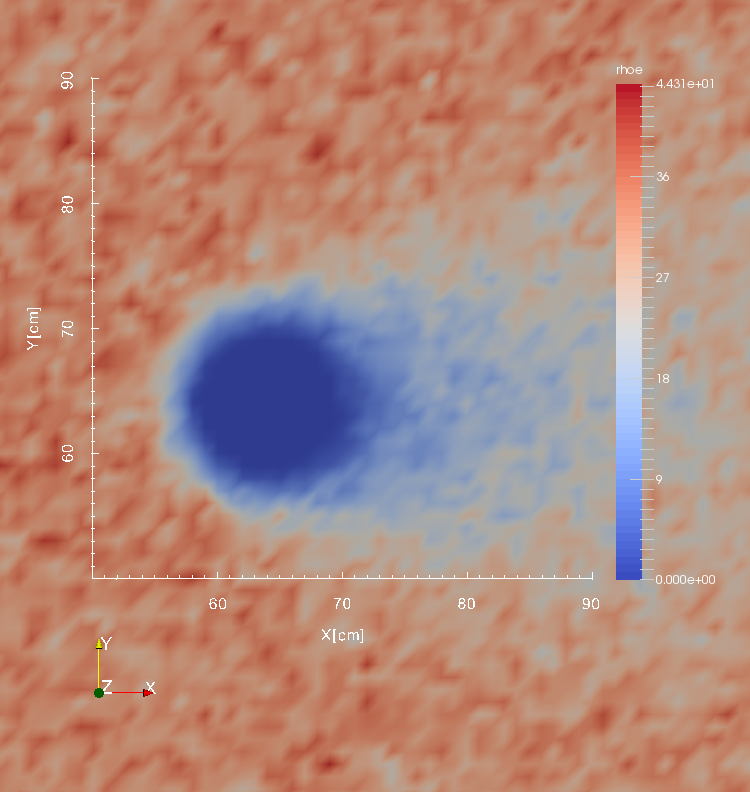
\includegraphics[width=0.99\linewidth]{rhoe_2sim_oslo_90D.png}
  \caption{Electron density}
  \label{fig:sub82}
\end{subfigure}
\caption{Cylinder with magnetic field at 90 degrees w.r.t the cylinder. Figure (\ref{fig:sub81}) and (\ref{fig:sub82}) shows the density of ions and electrons respectively. We can observe some asymmetry in the wake, slightly more than the simulation with 45 degrees.}
\label{fig:8}
\end{figure}

% Potential cylindere M2 with B90
\begin{figure}[H]
\centering
\begin{subfigure}{.5\textwidth}
  \centering
  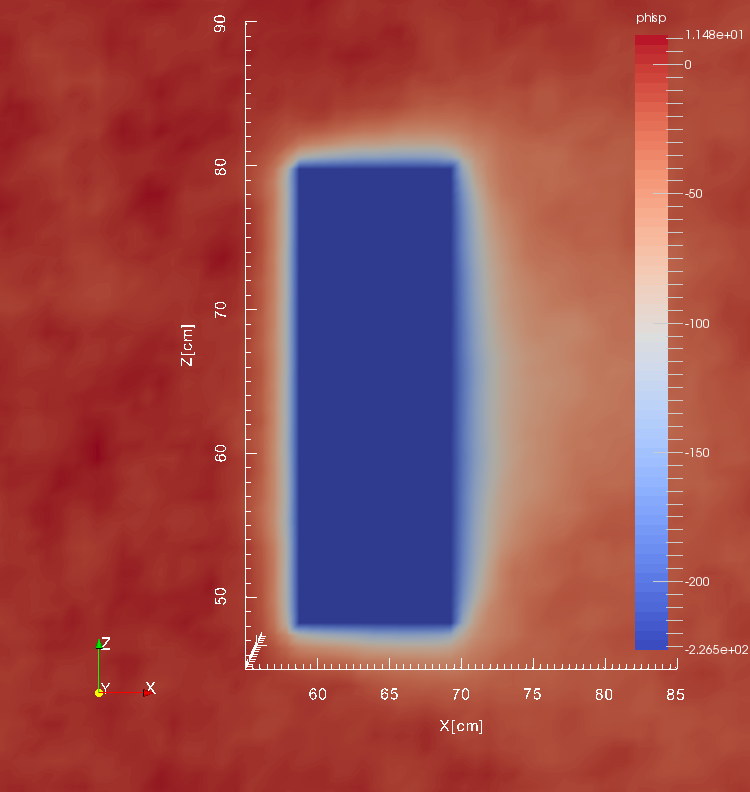
\includegraphics[width=\linewidth]{phis_2sim_oslo_B50.png}
  \caption{Electric potential}
  \label{fig:sub91}
\end{subfigure}%
\begin{subfigure}{.5\textwidth}
  \centering
  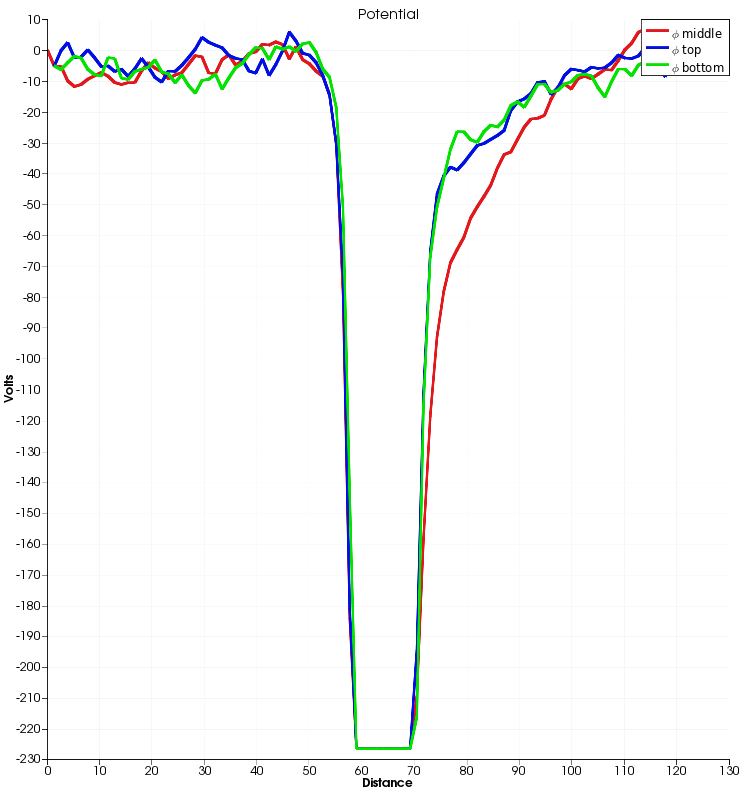
\includegraphics[width=\linewidth]{phispot_2sim_oslo_B50.png}
  \caption{Potential curve}
  \label{fig:sub92}
\end{subfigure}
\caption{Electric potential for a cylinder in a plasma flowing in the x-direction at $M=2$ and with a magnetic field perpendicular to the objects longitudinal direction. (\ref{fig:sub91}) is made by doing a cut through the center in the $xz$-plane. (\ref{fig:sub92}) is made by taking a cut through the center of the rectangle parallell with the x-axis.}
\label{fig:9}
\end{figure}

% Elevtrical currents, B0, j1 j2
\begin{figure}[H]
\centering
\begin{subfigure}{.5\textwidth}
  \centering
  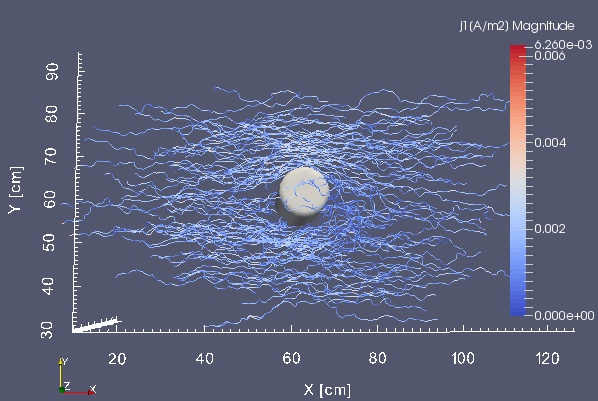
\includegraphics[width=\linewidth]{zoom/j1_Z(zoom).png}
  \caption{Electron current}
  \label{fig:sub101}
\end{subfigure}%
\begin{subfigure}{.5\textwidth}
  \centering
  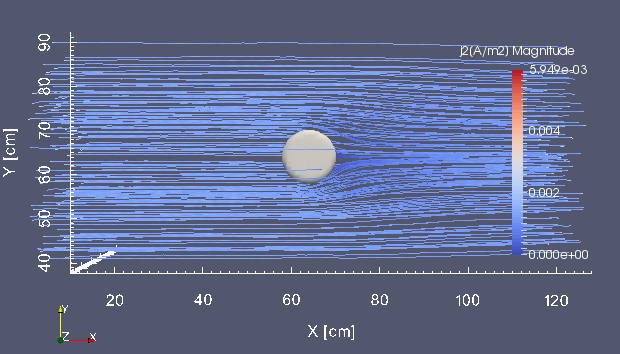
\includegraphics[width=\linewidth]{zoom/j2_Z(zoom).png}
  \caption{Ion current}
  \label{fig:sub102}
\end{subfigure}
\caption{Electron and ion currents in the $xy$-plane seen from above. No cut was made. Magnetic field at 0 degrees}
\label{fig:10}
\end{figure}

% Electrical currents, B45, j1 j2
\begin{figure}[H]
\centering
\begin{subfigure}{.5\textwidth}
  \centering
  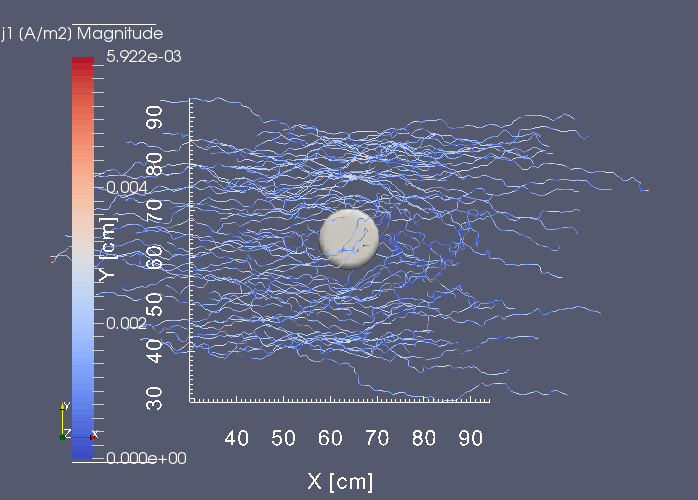
\includegraphics[width=\linewidth]{zoom_png/j1_zoom.png}
  \caption{Electron current}
  \label{fig:sub111}
\end{subfigure}%
\begin{subfigure}{.5\textwidth}
  \centering
  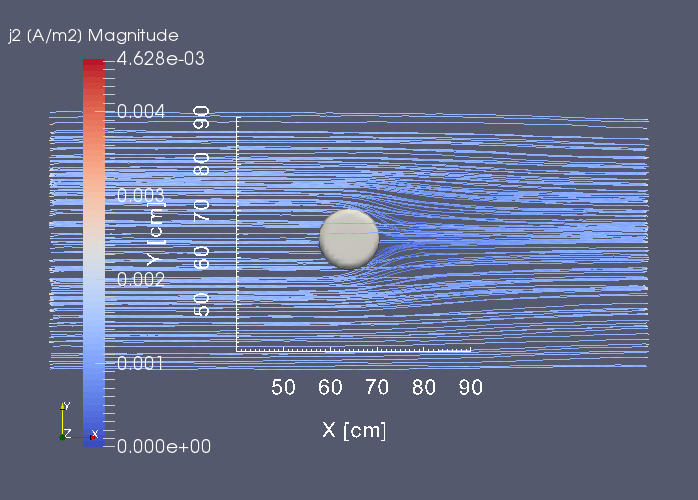
\includegraphics[width=\linewidth]{zoom_png/j2_zoom.png}
  \caption{Ion current}
  \label{fig:sub112}
\end{subfigure}
\caption{Electron and ion currents in the $xy$-plane seen from above. No cut was made. Magnetic field at 45 degrees.}
\label{fig:11}
\end{figure}



\begin{multicols}{2} % Two-column layout throughout the main article text

\section{Discussion}
This section first addresses the wake behind the rocket in the case of magnetic field degree is 0. Secondary, the discussion continues with the comparison where the magnetic field is rotated 0, 45 and 90 degrees to the z-axis.\\
\indent In figure (\ref{fig:sub51}) we can see the rocket potential falls into the negative.
The electron's motion is more dynamic than the ion's because of the thermal temperature.
The ratio of $Te/Ti$ is $1.5$. Then electron's collision probability is higher than the ion's. Hence the rocket potential becomes negative.
The rocket potential also affects the wake. If the rocket potential is neutral, the ion trajectory behind the rocket form straight lines, but negative potential attaches ions behind the rocket and forms the ion's wake.
In the case of electrons, magnetic field affects the wake form strongly.
The Larmor radius is calculated by $R_l = mv/qB$ 
In this case, the electron's Larmor radius is very small, and thereby trapped by the vertical magnetic field.
And the thermal motion also disturbes the wake form.
The random probability to penetrate behind the rocket is correlated to the thermal motion of the electrons, in other words, the fluctuation by the thermal motion of the electron is higher than that of the ion. Another way to see this is to compare
the mass of the electron with the ion and we will see that the electron is much lighter, thereby reaching supersonic speed
while the ion propagates with subsonic speed. We can see the sheath forming as a result of the ambient electron flux compared to the ambient ions.




%----------------------------------------------------------------------------------------
%	REFERENCE LIST
%----------------------------------------------------------------------------------------

\begin{thebibliography}{99} % Bibliography - this is intentionally simple in this template

\bibitem{EMSES}
  Yohei Miyaki, Hideyuki Usui
  \emph{New electromagnetic particle simulation code for the analysis of spacecraft-plasma
interactions},
Physics of Plasmas (1994-present) 16,
062904 (2009); doi: 10.1063/1.3147922,

\bibitem{melandso}
  Melands{\o}, F and Goree, J,
  \emph{Polarized supersonic plasma flow simulation for charged bodies such as dust particles and spacecraft},
  Physical Review E,
  Volume 52,
  no. 5,
  1995,
  APS
\bibitem{wang}
  Wang, J and Hastings, DE,
  \emph{Ionospheric plasma flow over large high-voltage space platforms. II: The formation and structure of plasma wake},
  Physics of Fluids B: Plasma Physics (1989-1993),
  volume 4,
  no. 6,
  1992,
  AIP Publishing

\bibitem{miloch}
  Miloch, Wojchiech J,
  \emph{Wake effects and Mach cones behind objects},
  PLASMA PHYSICS AND CONTROLLED FUSION,
  2010,
  IOP Publishing

\bibitem{holmstrom}
  M. Holmstrom, S. Fatemi, Y. Futaana, and H. Nilsson,
  \emph{The interaction between the Moon and the solar wind},
  Earth Planets Space,
  volume 64,
  page 237-245,
  2012

\bibitem{allen}
  Allen, J E,
  \emph{On supersonic plasma flow around an obstacle},
  J. Plasma Physics,
  page 1 of 5,
  Cambridge University Press,
  2012

\bibitem{meyer-vernet}
  Meyer-Vernet, N,
  \emph{Rocket spin effects on the current collected by a cylindrical probe in the ionosphere },
  Journal of geophysical research,
  vol. 81,
  no. 4,
  february 1,
  1976

\bibitem{guio}
  Guio, P., Miloch, W. J., Pecseli, H. L. and Trulsen, J.,
  \emph{Patterns of sound radiation behind pointlike charged obstacles in plasma flows},
  Phys. Rev. E,
  vol. 78,
  july 2008,
  American Physical Society

\end{thebibliography}

%----------------------------------------------------------------------------------------
\end{multicols}


\end{document}